\documentclass[10pt,a4paper]{article}
\usepackage[margin=21mm,headheight=15pt]{geometry}
\usepackage[T1]{fontenc}
\usepackage{lmodern,amsmath,amssymb,tikz,graphicx,hyperref,fancyhdr,enumitem}
\usetikzlibrary{arrows.meta,positioning,calc,decorations.pathmorphing}
\definecolor{ink}{RGB}{20,53,78}
\hypersetup{colorlinks=true,urlcolor=ink,linkcolor=ink}
\setlength{\parindent}{0pt}\setlength{\parskip}{5pt}
\emergencystretch=3em
\pagestyle{fancy}\fancyhf{}\fancyfoot[C]{\thepage}
\renewcommand{\headrulewidth}{.3pt}
\newcommand{\task}[2]{\par\medskip{\color{ink}\Large\bfseries #1. #2}\par\smallskip}
\newcommand{\answer}{\par\smallskip\textbf{Worked reasoning.} }
\setlist[enumerate]{label=\textbf{(\alph*)},leftmargin=7mm,itemsep=7pt}
\begin{document}
\fancyhead[L]{\small Control of Dynamical Systems}
\fancyhead[R]{\small Laboratory 07}
{\color{ink}\LARGE\bfseries Laboratory 07}\par
{\large A feedback loop with a communication delay}\par
\textbf{Exercise sheet -- five integrated problems}\par
{\small\textbf{Evidence boundary.} Original hypothetical scenarios. Derive, calculate and justify decisions; every numerical record is synthetic. Figures are conceptual and not to scale.}
\smallskip\textbf{Shared nominal data.} Nominal loop: $L(s)=8e^{-Ts}/[s(s+3)]$, unity negative feedback, and ideal constant delay $T$. Exact-delay results and rational Pad\'e approximations must be distinguished.
\task{1}{A remotely observed actuator}
A sensor observes a moving carriage through a communication link. Use the declared delay-free loop and distinguish its physical dynamics from the additional time spent transporting information.
\begin{center}\resizebox{\ifdim\width>.98\linewidth.98\linewidth\else\width\fi}{!}{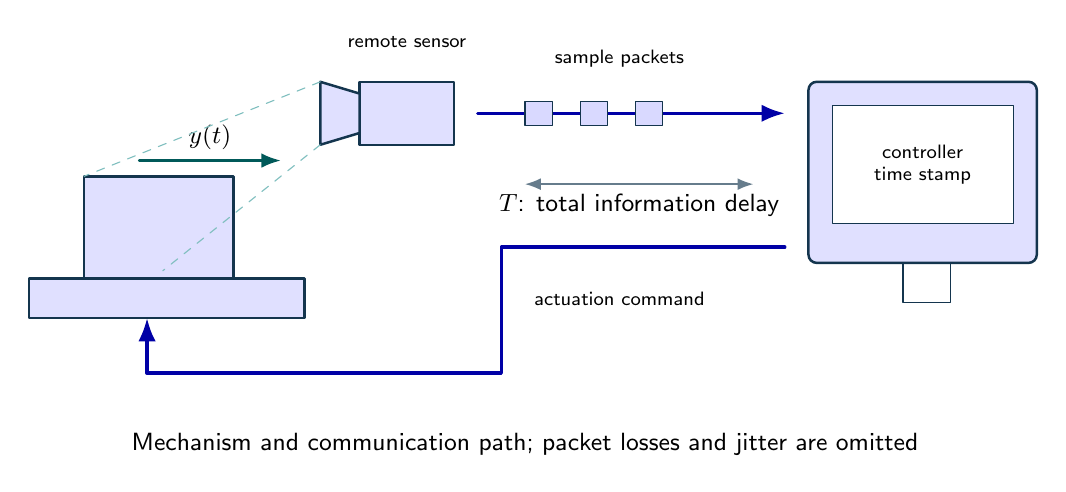
\begin{tikzpicture}[
font=\sffamily\small,>=Latex,line cap=round,line join=round,
wall/.style={draw=ink,line width=1.2pt,fill=blue!5},
water/.style={fill=cyan!25,draw=none},
metal/.style={draw=ink,fill=blue!12,line width=.9pt},
flow/.style={->,draw=blue!65!black,line width=1.2pt},
heat/.style={->,draw=orange!85!black,line width=1.1pt},
measure/.style={->,draw=teal!70!black,line width=.9pt},
dim/.style={<->,draw=ink!65,line width=.6pt},
spring/.style={draw=ink,decorate,decoration={coil,aspect=.5,segment length=4pt,amplitude=3pt}},
wire/.style={draw=ink,line width=1pt},
lab/.style={align=center,font=\sffamily\small},
smalllab/.style={align=center,font=\sffamily\scriptsize}]

\draw[metal](.5,1)rectangle(4,1.5);
\draw[metal](1.2,1.5)rectangle(3.1,2.8);
\draw[measure](1.9,3)--(3.7,3)node[midway,above]{$y(t)$};
\draw[metal](4.7,3.2)rectangle(5.9,4);
\draw[metal](4.7,3.35)--(4.2,3.2)--(4.2,4)--(4.7,3.85)--cycle;
\draw[teal!50,dashed](4.2,3.2)--(2.2,1.6)(4.2,4)--(1.2,2.8);
\node[smalllab]at(5.3,4.5){remote sensor};
\draw[metal,rounded corners=3pt](10.4,1.7)rectangle(13.3,4);
\draw[fill=white,draw=ink](10.7,2.2)rectangle(13,3.7);
\draw[ink](11.6,1.7)--(11.6,1.2)--(12.2,1.2)--(12.2,1.7);
\node[smalllab]at(11.85,2.95){controller\\time stamp};
\draw[flow](6.2,3.6)--(10.1,3.6);
\foreach \x in {6.8,7.5,8.2}{\draw[fill=blue!15,draw=ink](\x,3.45)rectangle++(.35,.3);}
\node[smalllab]at(8,4.3){sample packets};
\draw[flow](10.1,1.9)--(6.5,1.9)--(6.5,.3)--(2,.3)--(2,1);
\node[smalllab]at(8,1.25){actuation command};
\draw[dim](6.8,2.7)--node[below]{$T$: total information delay}(9.7,2.7);
\node[lab]at(6.8,-.6){Mechanism and communication path; packet losses and jitter are omitted};
\end{tikzpicture}
}\par{\small A remote mechanism sends measurements and receives commands through a communication path. The model combines those latencies into one ideal constant delay; the drawn packet train is not an experimental record.}\end{center}
\begin{enumerate}
\item The loop is $L_0(s)=8/[s(s+3)]$ with unity negative feedback. Derive its closed-loop poles, natural frequency and damping ratio.
\item Find the unique positive gain crossover of $L_0$. Show why an ideal pure delay $e^{-sT}$ does not change this crossover.
\item Write the exact delayed closed-loop characteristic equation. Explain why the delay-free second-order poles or any finite-order approximation do not list all modes of the delayed system.
\end{enumerate}
\vfill{\small\textbf{Submission.} Show the model, intermediate reasoning, units and a conclusion addressing the stated requirements.}

\newpage
\task{2}{Allocating a finite phase budget}
The loop must retain a stated phase margin after communication, computation and actuation delays. Budget the total delay rather than considering each component separately.
\begin{enumerate}
\item Calculate the nominal phase margin and the first positive pure-delay boundary. Express the formulas exactly before giving approximate values.
\item Find the maximum constant delay that retains at least a 30 degree phase margin. Compare it with delays of 0.1 s and 0.3 s.
\item Assume constant pure delays of 0.12 s, 0.04 s, 0.02 s and 0.01 s in successive stages. Determine whether their combined delay satisfies the 30-degree requirement and calculate the remaining unused delay allowance.
\end{enumerate}
\vfill{\small\textbf{Submission.} Show the model, intermediate reasoning, units and a conclusion addressing the stated requirements.}

\newpage
\task{3}{How a low-order delay approximation can overstate tolerance}
Compare the exact phase contribution with a first-order rational approximation. Use the comparison to audit a claimed stability boundary.
\begin{center}\resizebox{\ifdim\width>.98\linewidth.98\linewidth\else\width\fi}{!}{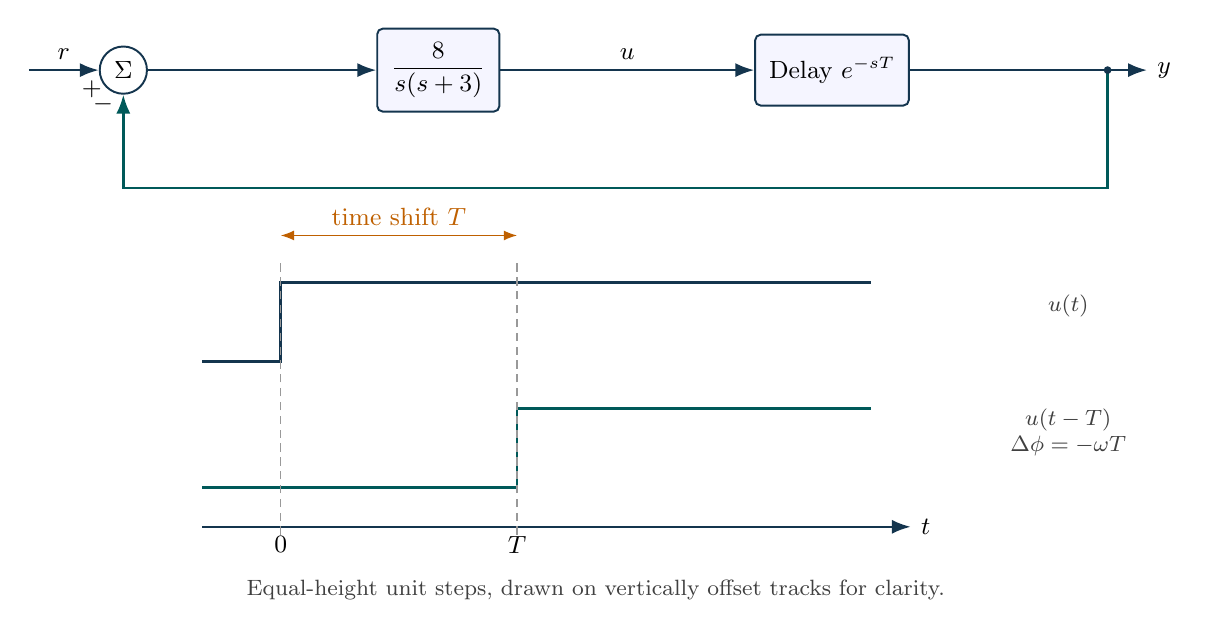
\begin{tikzpicture}[x=1cm,y=1cm,>=Latex,font=\small,
block/.style={draw=ink,fill=blue!4,rounded corners=2pt,minimum height=9mm,align=center,line width=.7pt,inner sep=5pt},
sum/.style={circle,draw=ink,fill=white,minimum size=6mm,inner sep=0pt,line width=.7pt},
sig/.style={->,draw=ink,line width=.85pt},
fb/.style={->,draw=teal!70!black,line width=.85pt},
dist/.style={->,draw=orange!75!black,line width=.85pt},
tap/.style={circle,fill=ink,inner sep=1.4pt},
note/.style={font=\footnotesize,align=center,text=black!75}]

\node[sum](e)at(1,2.1){$\Sigma$};
\node[block](g)at(5,2.1){$\dfrac{8}{s(s+3)}$};
\node[block](d)at(10,2.1){Delay $e^{-sT}$};
\draw[sig](-.2,2.1)--node[above]{$r$}node[pos=.9,below]{$+$}(e);
\draw[sig](e)--(g);\draw[sig](g)--node[above]{$u$}(d);
\draw[sig](d)--(14,2.1)node[right]{$y$};
\draw[fb](13.5,2.1)--(13.5,.6)--(1,.6)--node[pos=.9,left]{$-$}(e);
\fill[ink](13.5,2.1)circle(1.4pt);
\draw[sig](2,-3.7)--(11,-3.7)node[right]{$t$};
\draw[line width=1pt,draw=ink](2,-1.6)--(3,-1.6)--(3,-.6)--(10.5,-.6);
\draw[line width=1pt,draw=teal!70!black](2,-3.2)--(6,-3.2)--(6,-2.2)--(10.5,-2.2);
\draw[densely dashed,black!40](3,-3.8)--(3,-.35)(6,-3.8)--(6,-.35);
\node[below]at(3,-3.7){$0$};\node[below]at(6,-3.7){$T$};
\draw[<->,orange!75!black](3,0)--node[above]{time shift $T$}(6,0);
\node[note]at(13,-.9){$u(t)$};
\node[note]at(13,-2.5){$u(t-T)$\\$\Delta\phi=-\omega T$};
\node[note]at(7,-4.5){Equal-height unit steps, drawn on vertically offset tracks for clarity.};

\end{tikzpicture}
}\par{\small Constant pure delay shifts a signal in time and contributes frequency-dependent phase lag. The sketch shows ideal steps, not experimental records.}\end{center}
\begin{enumerate}
\item Write the first-order Pade approximation of $e^{-sT}$. Locate its pole and zero and explain why the right-half-plane zero does not mean the exact delay has a finite unstable zero.
\item At the crossover of this loop, compare exact delay phase with first-order Pade phase for $T=0.3$ s. Derive the sign of the approximation error for any positive frequency.
\item Derive the first-order Padé estimate of the delay boundary at the unchanged crossover, and compare it symbolically with the exact boundary. State the direction of the error without relying on a plot.
\end{enumerate}
\vfill{\small\textbf{Submission.} Show the model, intermediate reasoning, units and a conclusion addressing the stated requirements.}

\newpage
\task{4}{Sensor dynamics invalidate a previously acceptable delay budget}
A sensor lag is added after the original delay requirement was checked. Reassess the uncertain-delay interval using the modified loop.
\begin{enumerate}
\item Add sensor $1/(0.1s+1)$ to the delay-free loop. Calculate its magnitude and phase at the old crossover. Explain what must be recomputed before stating an exact new delay budget.
\item Suppose the constant delay is uncertain in $[0.12,0.18]$ s. Find the smallest phase margin across this interval and decide whether all frozen-delay models meet a 30 degree margin. Does the result automatically cover arbitrary time-varying jitter?
\item For the added sensor, derive the equation for the new positive crossover. Recompute the worst frozen-delay phase margin over $T\in[0.12,0.18]$ and decide whether the 30-degree requirement still holds.
\end{enumerate}
\vfill{\small\textbf{Submission.} Show the model, intermediate reasoning, units and a conclusion addressing the stated requirements.}

\newpage
\task{5}{Trading loop speed for delay tolerance and numerical fidelity}
Reduce loop gain and compare exact-delay simulation with an approximation. Verify both the control tradeoff and the time indexing of the numerical model.
\begin{enumerate}
\item Replace numerator 8 by 4. Derive the new crossover and delay boundary and compare the control-design tradeoff.
\item An exact delayed plant response is zero before delay T when initial conditions are zero. Explain why a finite-order Pade simulation may respond immediately. Describe a reproducible numerical check for a delay-buffer simulation.
\item Represent a 0.605 s delay using a 0.01 s step and integer-sample rounding. Bound the resulting delay error and its phase error at the new crossover. Propose a grid that represents the stated delay exactly.
\end{enumerate}
\vfill{\small\textbf{Submission.} Show the model, intermediate reasoning, units and a conclusion addressing the stated requirements.}

\end{document}
